%!TEX root = main.tex
\subsection{Methodology}
        We apply the so-called transcript method to solve our (OCP).
    This method transforms the underlying problem of
    optimizing functional governed by a differential equation into a
    finite-dimensional optimization problem with restrictions. To fix ideas,
    let $x$, $u$ respectively denote state and control, and consider the
    optimal control problem
    \begin{equation*}
        \begin{aligned}
                & \min J(x(\cdot), u(\cdot)) = g_0(T, x(T))
                & \text{Functional cost}
            \\
                & \dot{x} = f(t, x(t), u(t)),
                \quad\forall t \in [0, T],
                & \text{Dynamics}
            \\
                & u(t) \in \mathcal{U}[0, T] \text{for a.e. } t\in [0, T]
                & \text{Admissible controls}
            \\
                & g(x(t), u(t)) \leq 0
                & \text{Path constrain}
            \\
                & \Phi(x(0), x(T)) = 0
                & \text{Boundary conditions}.
        \end{aligned}
    \end{equation*}
        Then, transcription methods transform this infinite-dimensional
    optimization problem into a finite dimension problem (NLP) via
    discretization of dynamics, state, and control.  For example, if we
    employ the Euler method with a discretization of $N$ constant steps with
    size $h$, then we can solve
        \begin{equation}
            \label{eqn:nlp}
            \begin{aligned}
                    &\min g_0(t_N, x_N)
                \\
                    &
                        x_{i+1} = x_i + h f(x_i, u_i),
                    & i = 0, \dots, N - 1
                \\
                    &
                        u_i \in \mathcal{U},
                    & i = 0, \dots, N
                \\
                    &
                        g(x_i, u_i) \leq 0,
                    & i = 0, \dots, N
                \\
                    &
                    \Phi(x_0, x_N) = 0,
                    &i = 0, \dots, N,
            \end{aligned}
        \end{equation}
    where $x_i \approx x(t_i)$,
    $u_i \approx u(t_i)$ in the grid
    $$
        \left\{
            t_0 = 0,\quad
            t_i = i h \ (i=1,\dots, N-1),\quad
            t_N = T
        \right\}.
    $$
    Let $Y = \{x_0, \dots, x_N, u_0,\dots u_N\}$.
    Thus \Cref{eqn:nlp} defines a nonlinear programming problem on the
    discretized state and control variables of the form
    \begin{equation}
        \label{eqn:nlp_form}
        \begin{aligned}
            &
            \min F(Y)
        \\
        \text{such that} &
        \\
            &
            LB \leq C(Y) \leq UB .
        \end{aligned}
        %\tag{NLP}
    \end{equation}
    %
        The numerical analysis and design of transcript methods is a well
    established  and active research numerical field. There is a vast
    literature about robust methods and recently, implementations have been
    developed in vogue languages like Julia
    \cite{DunningHuchetteLubin2017, LubinDunningIJOC}, Python \cite{libcmaes},
    Matlab \cite{matlabOpt}, and others. We refer the reader to
    \cite{Betts2001,Seywald1993} for a more systematic discussion.

        Our simulations rely on the \verb|Bocop| package
    \cite{Bocop,BocopExamples} to solve our (OCP). Bocop is part of the
    development of the INRIA-Saclay initiative for open source optimal control
    toolbox and supported by the team Commands. BOCOP solves the NLP problem in
    \Cref{eqn:nlp_form} by the well known software \textsc{Ipopt} and using
    sparse exact derivatives computed by ADOL-C.

        We provide in \cite{gitHub} a GitHub repository with all regarding R
    and Bocop sources. This repository also encloses data sources and python
    code to reproduce all reported figures.

\subsection{Simulation of hypothetical scenarios}
        We follow the guidelines reported by the WHO Strategic Advisory Group
    of Experts (SAGE) on Immunization Working Group on COVID-19 Vaccines
    modeling questions presented in \cite{sage2020}. According to this SAGE's
    document, we simulate scenarios to illustrate vaccination policies'
    response with a preventive vaccine. We aim to contrast the impact of the
    burden of COVID-19 mitigation regarding
    \begin{enumerate}[(\textbf{SCN}-1)]
        \item Optimal versus constant vaccination policies
        \item Vaccine efficacy
        \item Induced vaccine immunity
        \item Natural immunity
    \end{enumerate}

    \added[id=SDIV, comment = cites]{
        We consider vaccine profiles\textemdash efficacy and induced vaccine
    immunity\textemdash compatible with  the firms Pfizer-BioNTech,
    Moderna, Astra-Zeneca, Gamaleya Research Institute
    Johnson \& Johnson, Sinovac Biotech among others.
    Further, since reinfection and induced vaccine immunity parameters remain
    unavailable, we see pertinent to explore the effect of plausible settings.
    }
%
    \begin{rmk}
        Optimal vaccination policy implies that number of doses per unit time
        described by

        $$
            (\psi_{V}+u_V(t))(S(t)+E(t)+I_A(t)+R(t))
        $$
        mitigates the outbreak in optimal form, where optimal is defined in
        terms of function $J$ (see \Cref{eqn:cost_functional}), that is
        minimizing years of life lost in DALYs.
        Counterfactual scenarios implies $u_V(t)=0$. Without vaccination
        scenarios we means $\psi_{V} + u_V(t)=0,  \ \forall t \in [0, T]$.
    \end{rmk}
%
    \begin{rmk}
        We assume positive prevalence of all epidemiological
        classes according to the following hypothesis:
        \begin{enumerate}[{(IC)}-1]
            \item
                The implemented initial conditions for our
                numerical experiments are
                hypothetical and not reflects the
                actual data reported by Mexico-City and Mexico-State
                health authorities. The initial conditions are taken such
                that an outbreak is on its growth phase
                (see \Cref{Fig:initial_conditions}).
            \item
                We suppose that around of \SI{30}{\percent}
                of the population is under Lockdown and is
                enclosed along with recovered class $R$. That
                is, $R(0)$ encircle mainly  children, senior,
                home office, people with low mobility and
                COVID-19 recovered individuals.
            \item
                Our numerical results are of
                qualitative nature and non necessarily sustain
                forecasting or follows the actual profile of the
                underlying COVID-19 pandemic data.
        \end{enumerate}
    \end{rmk}

    \begin{figure*}[h!]
        \centering
        \includegraphics[scale=1]{Figure_6.png%Figure_23.pdf
        }
        \caption{
            Hypothetical scenario when considering COVID-19 transmission
            dynamics without vaccination process. Blue line shows symptomatic
            prevalence dynamics. Red cross represents the initial date of
            simulations.
        }
        \label{Fig:initial_conditions}
    \end{figure*}

    \Cref{tbl:scene_parameters} encloses a brief description
    and parameter values regarding each scenario. The reader
    can also access the web
    \verb|Chart Studio Graph| of each figure regarding data and
    \verb|plotly| \cite{plotly} visual representation.
%
    \begin{table*}[tbh]
        \centering
        \begin{tabular}{%
                >{\centering}
                p{0.1\textwidth}
                p{0.23\textwidth}
                p{0.57\textwidth}
            }
            \toprule
            \textbf{Simulation Scene}
            & \textbf{\qquad Description}
            & \textbf{Set-up} \quad
            $(x_{coverage}, T, \varepsilon_{V}, \omega_{V}^{-1}, \sigma_{R}^{-1})$
            \\
            \midrule
            \textbf{(SCN-1)}
            &
            Likening between optimal and constant
            vaccination policies.
            &
            (%
            \SI{20}{\percent},
            \SI{180}{days},
            \SI{70}{\percent},
            \SI{730}{days},
            \text{lifelong}
            )
            \\
            \textbf{(SCN-2)}
            &
            Vaccine efficacy blow
            &
            (%
            \SI{50}{\percent}, %
            \SI{365}{days}, %
            $\left\{
            \SI{50}{\percent},
            \SI{70}{\percent},
            \SI{90}{\percent}
            \right\}
            $, %
            \SI{730}{days}, %
            \SI{180}{days}
            )
            \\
            \textbf{(SCN-3)}
            &
            Induced vaccine immunity period
            &
            (%
            \SI{50}{\percent}, %
            \SI{365}{days}, %
            \SI{90}{\percent},
            $\left\{
            \SI{180}{days},
            \SI{365}{days},
            \SI{730}{days}
            \right\}
            $, %
            \SI{365}{days}%
            )
            \\
            \textbf{(SCN-4)}
            &
            Natural immunity period
            &
            (%
            \SI{50}{\percent}, %
            \SI{365}{days}, %
            \SI{90}{\percent}, %
            \SI{730}{days}, %
            $
            \left\{
                \SI{90}{days},
                \SI{180}{days},
                \SI{365}{days}
            \right\}
            $%
            )
            \\
            \bottomrule
        \end{tabular}
        \caption{
            Setup parameters for counterfactual and response scenarios. See
            \Cref{tbl:fixed_parameters} for the rest of parameters.}
        \label{tbl:scene_parameters}
    \end{table*}
%

    To perform the simulations corresponding to the scenarios presented in
\Cref{tbl:scene_parameters}, we fix the parameter values as in
\Cref{tbl:fixed_parameters-OCM}.
%
\begin{table*}[tbh]
    \begin{center}
        \begin{tabular}{rc@{}c}
            \toprule
            \multicolumn{3}{c}{\textbf{Parameters values}}
            \\
            \midrule
            \\
                & \multicolumn{2}{c}{\textbf{(SCN-1)--(SCN4)}}
                \\
                \cmidrule{2-3}
                \\
                $\beta_S$, $\beta_A$, $\alpha_{S}$, $\alpha_{A}$, $\sigma_{E}$,
                $\mu$, $\theta$, $p$
                & \multicolumn{2}{c}{\Cref{tbl:fixed_parameters}}
            \\
                $a_D$, $a_S$, $\kappa$, $B$
                & \multicolumn{2}{c}{\Cref{tbl:ocp_parameters_description}}
            \\

            \\
                & \textbf{(SCN-1)}
                & \textbf{(SCN-2)}--\textbf{(SCN-4)}
            \\
                \cmidrule{2-3}
                %\cmidrule{3-3}
            %\\
%                \cmidrule{3-3}
%            \\
            $\psi_{V}$
                & \num{0.00123969}
                & \num{0.00189903}
            \\
                $u_{min}$
                & \num{-0.000619845}
                & \num{-0.00094952}
            \\
                $u_{max}$
                & \num{0.00619845}
                & \num{0.00474758}
            \\
            \bottomrule
        \end{tabular}
        \caption{%
            Fixed parameters values of system in
            \Cref{eqn:optimal_control_problem}.}
        \label{tbl:fixed_parameters-OCM}
    \end{center}
\end{table*}
%
\section*{Optimal Versus Constant Vaccination Policies: (SCN-1)}
        To fix ideas, we display in
        \Cref{fig:lifelongvaccinationpolicies,%
        fig:lifelongvaccinationpoliciesOutbreak}
    the counterfactual scenario regarding no intervention. We
    contrast a constant vaccination policy (CP) and optimal vaccination
    policy (OP) with a vaccine profile of efficacy
    $\varepsilon_V = \SI{70}{\percent}$, vaccine-induced immunity
    $\omega_V^{-1} = \SI{730}{days}$ and a campaign for \SI{20}{\percent}
    of coverage at \SI{180}{days}. \Cref{fig:lifelongvaccinationpolicies}
    suggests that the OP improves CP vaccination policy response according to
    the disease burden due to mortality, and morbidity.
    \Cref{fig:lifelongvaccinationpoliciesOutbreak} confirms this improvement by
    comparing disease dynamics with and without vaccination. We observe CP and
    OP reduce disease levels. Although both campaigns administrate the same
    number of vaccine doses, OP vaccination implies fewer deaths and
    symptomatic cases.
    \deleted[id=SDIV, comment= Fix this paragraph]{Figure 3 %
        %\Cref{fig:lifelongvaccinationpolicies}
    shows a scenario whit
    $R_0>1$. The underlying vaccine reproductive number $R_V$
    remains below to $R_0$. This Figure illustrates the strong relation between disease mitigation, vaccine efficacy $(\varepsilon_{V})$,
    and vaccination rate $(\psi_{V})$. Further, given a dynamic
    without vaccine intervention and $R_0>1$, $R_V$ projects a
    minimal vaccination rate to drive this dynamic to the disease-free state
    but subject to vaccines with particular efficacy.}
    %
    \begin{figure*}[tbh!]
        \centering
        \includegraphics[scale=1]{Figure_7.png}
        \caption[Effect of the vaccination policy on the burden COVID-19]{%
        Effect of the vaccination policy on the burden COVID-19 for a 20\%
        coverage at time horizon of half year.
        (A) Vaccination policies' response regarding constant ($\psi_V$)
        and optimal ($\psi_V+u_V(t)$)  vaccination rates in the burden of
        COVID-19 quantified in DALYs. (B) Evolution of the
        vaccination covering according to each policy.
        (C) Vaccination schedule for each vaccination policy.
        Blue translucent color corresponds to policies with constant
        vaccination rate \num{0.00123969}. Green tone is related to the
        optimal vaccination policy. For counterfactual reference (panel A),
        black line-gray shade represents the burden of COVID-19 without
        vaccination.
        See \href{https://plotly.com/~MAAZ/366/}{%
                https://plotly.com/~MAAZ/366/}
        for plotly visualization and data.
        }
        \label{fig:lifelongvaccinationpolicies}
    \end{figure*}
    \begin{figure*}[tbh!]
        \centering
        \includegraphics[scale=1]{Figure_8.png}
        \caption[Effect of the vaccination policy on outbreak evolution.]{
        Effect of the vaccination policy on outbreak evolution.
        (A) Optimal vaccination policy reaches a better response in mitigating
        symptomatic cases than a policy with a constant vaccination rate.
        (B) Gray and blue shaded translucent regions denote the number of
        saved lives per \SI{100000}{inhabitants}.
        The optimal vaccination rate (grey-blue) improves the number of saved
        lives per \SI{100000}{inhabitants} of the constant rate $\psi_V$.
        Data and web visualization in
        \href{%
            https://plotly.com/~MAAZ/370/
        }{https://plotly.com/~MAAZ/370/}.
        }
        \label{fig:lifelongvaccinationpoliciesOutbreak}
    \end{figure*}
%
    \section*{Vaccine Efficacy (SCN-2)}
        \comment[id=SDIV]{Fix.
            Say that has been approved developments in
            Mexico
        }
        In February 2021, multiple vaccines have been rolled out to prevent
        COVID-19 disease. \Cref{tbl:vaccine-efficacy-portfolio} contains
        information on developments that we consider relevant to explore a wide
        range of plausible vaccine-efficacies.
        \begin{table}[htb]
            \centering
            \begin{tabular}{%
                p{3cm}
                p{2cm}
                p{3.5cm}
                P{2cm}
            }
            \toprule
            \textbf{Developer} &
            \textbf{Vaccine Name} &
            \textbf{Vaccine Efficacy \%, (95\% CI)} &
            %\textbf{Status} &
            \textbf{Reference}
                \\
                 \midrule
                \\
                    Pfizer-BioNTech
                        & BNT162b2
                        & \num{95} (\num{90.3}–\num{97.6})
                        %& Approved for emergency use in the USA, Mexico,
                        % Germany, UK, and other countries
                        & \cite{vaccine_tracker2020}
                \\
                    Gamaleya Institute
                        & Sputnik V
                        & \num{91.6} (\num{85.6}–\num{95.2})
                        %& Early use in Russia. Emergency use Mexico an other
                        %countries.
                        & \cite{Logunov2021}
                \\
                    Oxford University-AztraZeneca
                        & AZD1222
                        & \num{74.6} (\num{41.6}-\num{88.9})
                        %& Approved for emergency use in the USA, Mexico,
                        & \cite{Emary2021}
                \\
                    Johnson \& Johnson
                        & Ad26.COV2.S
                        & \SI{72}{\percent}
                        %& Approved for emergency use in the USA, Mexico,
                        & \cite{johnsonandjohnson}
                \\
                    Sinovac Biotech
                        & CoronaVac
                        & 50.4\%
                       % & Approved in China. Emergency use in Brazil, other
                       % countries.
                        &\cite{vaccine_tracker2020}
                \\
            \bottomrule
            \end{tabular}
            \caption{Vaccine efficacy of some
            to the platforms approved to emergency use.}
            \label{tbl:vaccine-efficacy-portfolio}
        \end{table}
%
    \begin{itemize}
        \item
            by Pfizer-BioNTec has
            95\% effectiveness (95\% CI, 90.3 to 97.6) \cite{Polack2020};
        \item
            Sputnik V by Gamaleya has
            91.6\% effectiveness (95\% CI 85.6–95.2) \cite{Logunov2021};
        \item
            AZD1222 by Oxford-48AstraZeneca has vaccine efficacy for
            different virus lineages with 74.6\% [95\% CI 41.6-88.9] and
            84 \% [95\% CI 70.7-91.4], respectively \cite{Emary2021};
        \item
            Ad26.COV2.S by Johnson \& Johnson has a vaccine's efficacy against
            moderate and severe disease ranged from one country to another:
            72\% in the US, 66\% in Latin America and 57\% in South Africa
            \cite{johnsonandjohnson};
        \item CoronaVac by Sinovac Biotech has 50.4\% effectiveness
            \cite{vaccine_tracker2020}.
    \end{itemize}

    \Cref{fig:efficiencyvaccineprofile,fig:efficiencyvaccineprofileOutbreak}
    display the optimal vaccination policy's response  according to three
    vaccines with different efficacy. \Cref{fig:efficiencyvaccineprofile}A
    displays COVID-19 burden in DALYs for policies with
    \SI{50}{\percent},
    \SI{70}{\percent},
    \SI{90}{\percent}
    vaccine-efficacies.
    Figures \ref{fig:efficiencyvaccineprofile}B-C also illustrate the effect
    of vaccine-efficacies on coverage and optimal vaccination policy
    respectively.
    \added[id=SDIV, comment={how?, be concise}]{
    We observe that vaccine-efficacy influences design optimal policy.}
    According to \SI{50}{\percent} coverage at a time horizon of
    \SI{1}{year}, \Cref{fig:efficiencyvaccineprofileOutbreak} displays an
    improvement of at least three times in the prevalence of symptomatic cases
    and saved lives concerning the uncontrolled
    outbreak. \Cref{fig:efficiencyvaccineprofileOutbreak} reflects this
    effect in the mitigation
    symptomatic prevalence (A) and
    the number of saved lives (B) shaded by the translucent
    grey (50\% vaccine efficacy), grey-blue (70\% vaccine efficacy), and
    grey-blue-red (90\% vaccine efficacy).
%
%------------------------------------------------------------------------------
% Vaccine efficacy gradient
%
    \begin{figure*}[htb]
        \centering
        \includegraphics[scale=1]{%
            Figure_9.png%./EfficiencyVaccineProfile_v2.png%
        }
        \caption[The response of COVID-19 to vaccine efficacy]{
            The response of COVID-19 burden to vaccine efficacy.
            (A) COVID-19 burden response quantified in DALYs per \SI{100000}{
            inhabitants}  to vaccines with efficacy of
            \SI{50}{\percent} (blue),
            \SI{70}{\percent} (red) and \SI{90}{\percent}(green).
            (B) Coverage evolution to reach \SI{50}{\percent} of the total
            population vaccinated.
            (C) Optimal vaccination doses schedule according to the
            different efficacies. See
            \href{https://plotly.com/~MAAZ/358/}{%
                https://plotly.com/~MAAZ/358/} for
            visualization and data.
        }
        \label{fig:efficiencyvaccineprofile}
    \end{figure*}
%
    \begin{figure*}[htb]
        \centering
        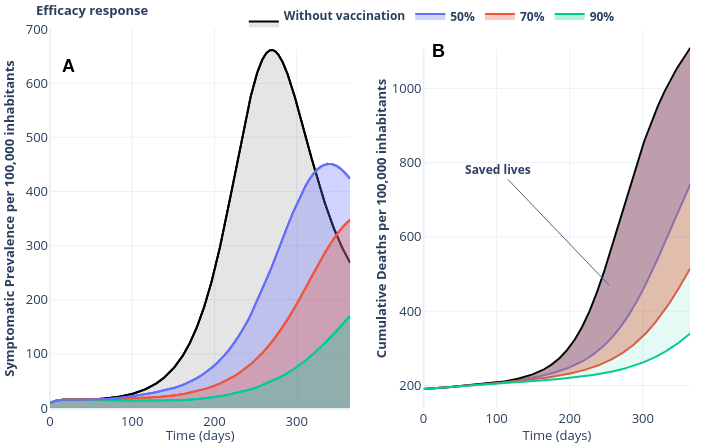
\includegraphics[scale=1]{%
            Figure_10.png%./EfficiencyVaccineProfileOutbreak.png%
        }
        \caption[The effect of vaccine efficacy over
            COVID-19 symptomatic prevalence and morbidity]{
            The effect of vaccine efficacy over COVID-19 symptomatic
            prevalence and morbidity.
            (A) Effect of vaccine-efficacy of
            \SI{50}{\percent} (blue), \SI{70}{\percent} (red)
             and \SI{90}{\percent} (green) on prevalence
             of symptomatic cases per \SI{100000}{inhabitants}.
            (B) Effect of vaccine-efficacy on the number of saved lives.
            See
            \href{https://plotly.com/~MAAZ/375/%
            }{https://plotly.com/~MAAZ/375/} for data and
            visualization.
        }
        \label{fig:efficiencyvaccineprofileOutbreak}
    \end{figure*}

\section*{Vaccine-induced immunity (SCN-3)}
    Vaccine response also is strongly related to its induced immunity
    \textemdash parameter that remains poorly understood
    \cite{Jeyanathan2020}.
    Here, we contrast two vaccines with different induced-immunity. Let
    denote by $vax_1$, $vax_2$, $vax_3$ vaccines with an induced-immunity
    capacity of a half, one, and two years, respectively, and common efficacy
    of \SI{90}{\percent}.
    Consider a vaccine camping of time horizon of one year and
    \SI{50}{\percent} coverage. Taking the same dynamics parameters, that is
    initial conditions, and baseline parameters, as in
    \Cref{tbl:fixed_parameters}, we explore a counterfactual scenario with an
    uncontrolled outbreak of $R_0 = \num{1.79493}$ and three controlled
    dynamics according to vaccines $vax_1$, $vax_2$, $vax_3$. Thus, according
    to these immunity parameters and factor defined in
    \Cref{eqn:mitigation_factor}, respectively, results
    $R_V^{[vax_1]} = \num{1.38555}$,
    $R_V^{[vax_2]} = \num{1.13913}$,
    $R_V^{[vax_3]} = \num{0.86756}$
    for vaccine immunities periods of a half, one, and two years. We display in
    \Cref{fig:induced_immunity_vaccine_profile} the response of the
    vaccines $vax_1$, $vax_2$ and $vax_3$. \az Since optimal vaccination
    policies are similar, \Cref{fig:induced_immunity_vaccine_profile} A
    suggests vaccine-induced immunity rate is not determinant in the
    vaccination schedule design. \st{Since in this  scenario set time
    horizon is of one year, the optimal policies follow similar schedules and
    imply similar gains in the number of years of life lost. Despite these
    similarities,} \za \Cref{fig:inducedimmunity_vaccine_outbreak}
    displays \az \st{in panel A dramatically gain respect to} a wide reduction
    of disease levels concerning the uncontrolled outbreak.
    \st{\textemdash since $R_V ^{[vax_2]}$ is near to one, prevalence
    fall-down more than five times and because $R_V ^{[vax_3]}$ is less that
    one, prevalence of symptomatic cases tends to zero with damped
    oscillations.
    Figure 13 also endorses this gain regarding
    saved lives (B). This gain is}
    It happens as a consequence of the vaccine reproduction number reductions.
    For this scenario, we observe that it is unnecessary to reduce $R_V$ below
     one to obtain notable mitigation. The disease level reduction
    represented by the shaded grey region (a half year),
    grey-green region (one years) and grey-green-red region (two years).
    \za
%
%-------------------------------------------------------------------------------
% Induced vaccine immunity gradient
    \begin{figure*}[htb]
        \centering
        \includegraphics[scale=1]{%
        Figure_11.png%InducedImmunityVaccineProfile%
        }
        \caption[
            Effect of Vaccine-induced immunity effect on the burden of COVID-19.
        ]{
            Effect of vaccine-induced immunity on the COVID-19 burden.
            (A) Effect on the burden of COVID-19 quantified in DALYs per
            \SI{100000}{inhabitants} due to vaccine-induced immunity of
            \SI{180}{days} (green), \SI{365}{days} (red) and 730 days (blue).
            (B) Coverage evolution to reach \SI{50}{\percent} of the total
            population vaccinated.
            (C) Optimal vaccination doses schedule according to the different
            vaccine-induced immunities. Visualization and data in
            \href{https://plotly.com/~MAAZ/407/}{%
                https://plotly.com/~MAAZ/407/
            }.
        }
        \label{fig:induced_immunity_vaccine_profile}
    \end{figure*}
    %
    \begin{figure*}[htb]
        \centering
        \includegraphics[scale=1]{Figure_12.png}
        \caption[Effect of vaccine-induced immunity
                on mitigation and saved lives of COVID-19 outbreak]{
            Effect of vaccine-induced immunity on mitigation and saved lives of COVID-19 outbreak.
            (A)  Effect of vaccine-induced immunity on mitigation of symptomatic prevalence per \SI{100000}{inhabitants}.
            (B) The number of saved lives. See
            \href{https://plotly.com/~MAAZ/416/}{%
                https://plotly.com/~MAAZ/416/}.
        }
        \label{fig:inducedimmunity_vaccine_outbreak}
    \end{figure*}
%------------------------------------------------------------------------------
\section*{Natural Immunity Hypothesis (SCN-4)}
%
     ``Reinfections raise questions about long-term immunity to
     COVID-19 and the prospects for a vaccine'',  reported
    Heidi Ledford in \cite{Ledford2020b}. Following this line, we
    display in \Cref{%
            fig:natural_recovering_profile,%
            fig:natural_recovering_outbreak}
    the vaccine's response with \SI{90}{\percent} efficacy and
    contrasting with  natural immunity periods of \SI{90}{days},
    \SI{180}{days}, and \SI{365}{days}. Here, the adjective ``natural''
    denotes the immunity that an individual develops after recovering from a
    previous bout of COVID-19 without vaccination.
    When implementing an optimal vaccination strategy, if natural
    immunity lasts one year, the burden of COVID-19 falls until around
    \SI{120}{DALYs}. We confirm this behavior in the prevalence of symptomatic
    cases and cumulative deaths, as displayed in
    \Cref{fig:natural_recovering_outbreak}. When natural immunity is
    \SI{365}{days}, the gain in mitigation concerning a natural immunity of
    \SI{90}{days} is at least \num{100} times, while the number of deaths
    with a natural immunity of \SI{90}{days} reach \num{845} cases per
    \SI{100000}{inhabitants}, in contrast, of \SI{206} when natural immunity is
    \SI{365}{days}. Thus, this simulation suggests that natural immunity
    plays a vital role in the controlled outbreak's behavior, which is
    consistent with the conclusions reported in \cite{Jeyanathan2020}.
%
    \begin{figure*}[tbh!]
        \centering
        \includegraphics[scale=1]{Figure_13.png}
        \caption[Effect of natural immunity on the burden of COVID-19]{
            Effect of natural immunity on the burden of COVID-19.
            (A) Effect on the burden of COVID-19 quantified in DALYs per
            100,000 inhabitants due to natural immunity of 90 days (red),
            180 days (blue) and 365 days (green).
            (B) Coverage evolution to reach \SI{50}{\percent} of the total
            population vaccinated.
            (C) Optimal vaccination doses schedule according to the different
            natural immunities. See
            \href{https://plotly.com/~MAAZ/402/}{%
                https://plotly.com/~MAAZ/402/}.
        }
        \label{fig:natural_recovering_profile}
    \end{figure*}
%
    \begin{figure*}[h!]
        \centering
        \includegraphics[scale=1]{Figure_14.png}
        \caption[Vaccine induced immunity profile.]{
            Effect of natural immunity on mitigation and saved lives of
            COVID-19 outbreak.
            (A) Effect of  immunity on mitigation of
            symptomatic prevalence per \SI{100000}{inhabitants}.
            (B) Number of saved lives. Plotly visualization and data in
            \href{https://plotly.com/~MAAZ/406/}{%
                https://plotly.com/~MAAZ/406/
            }.
        }
        \label{fig:natural_recovering_outbreak}
    \end{figure*}